\section{Overall Description}
\subsection{ Product perspective}
\subsubsection{UML Description}
The UML below describes at a high level the model of the system to be developed. It considers the basic
service together with the advanced function 1 and advanced function 2 previously specified. The UML does
not include every class that will be necessary to define the complete architecture of the system.
DREAM offers different functions beyond the basic service.
Here we can identify the main aspects related to DREAM:\newline

each farmland is shown by a specific point on the map and the policymaker by selecting each point can see the detail of farmland location, Progress status of each farmer, type of production, humidity, and used water. also, farmers can see their own status and insert faced problems in the system and production information. \newline


after login farmers should Insert the location of  their farmland and based on the type of production and weather forecast of these locations can suggest what crop to plant and which fertilized is better  to use also they can insert production detail while during crop growth and any related problem they face and by a related expert, system find the best solution and help them to Helps to keep going \newline


sensors that are located in the depth of land with defined distance, periodically send messages containing soil humidity and send to the network access point to gather and analyze and give specific alerts to necessity role\newline

an irrigation system  that is located all over the land with  defined distance, automatically measuring the used water send to the network access point to gather and analysis and give specific alert to necessity role \newline

policymaker assesses the performance of the farmer and determines the best and worst one with collected environmental data, such as the used amount of water that measure by irrigation system or humidity of soil that obtained from a sensor located in each farmland. Also, consider the type of production and location of land or even farmer faced a problem.\newline

\pagebreak
\subsection{state Charts}
Now we are going to analyze some critical aspects of the application, modeling their behaviors and showing the evolution over time of their states through appropriate state diagrams, which are reported below.
\newline

 \hspace{3cm} \footnotesize{ the state diagram mainly reports the change of state of class report }
 \begin{figure}[H]
%\centering
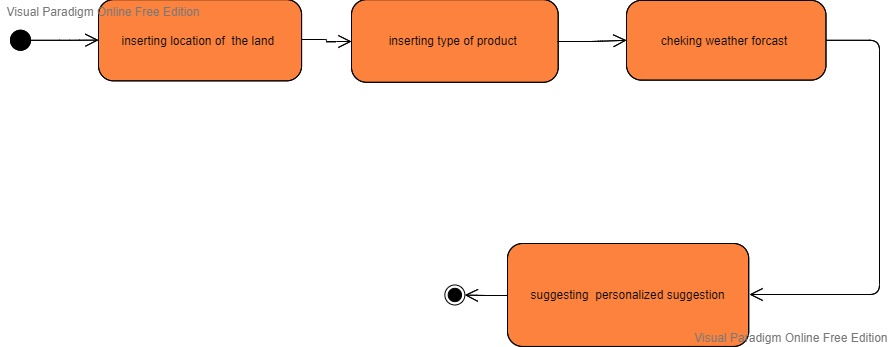
\includegraphics[width=1\textwidth]{figures/firstStateDiagram.jpg}
\caption{\label{fig:student } State Diagram 1 - inserting  of initial information to give personalized suggestion }
\end{figure}
in first diagram (figure1),we model the inserting of initial information by Farmer  showing the first step after login to give personalized suggestion 


 \begin{figure}[H]
%\centering
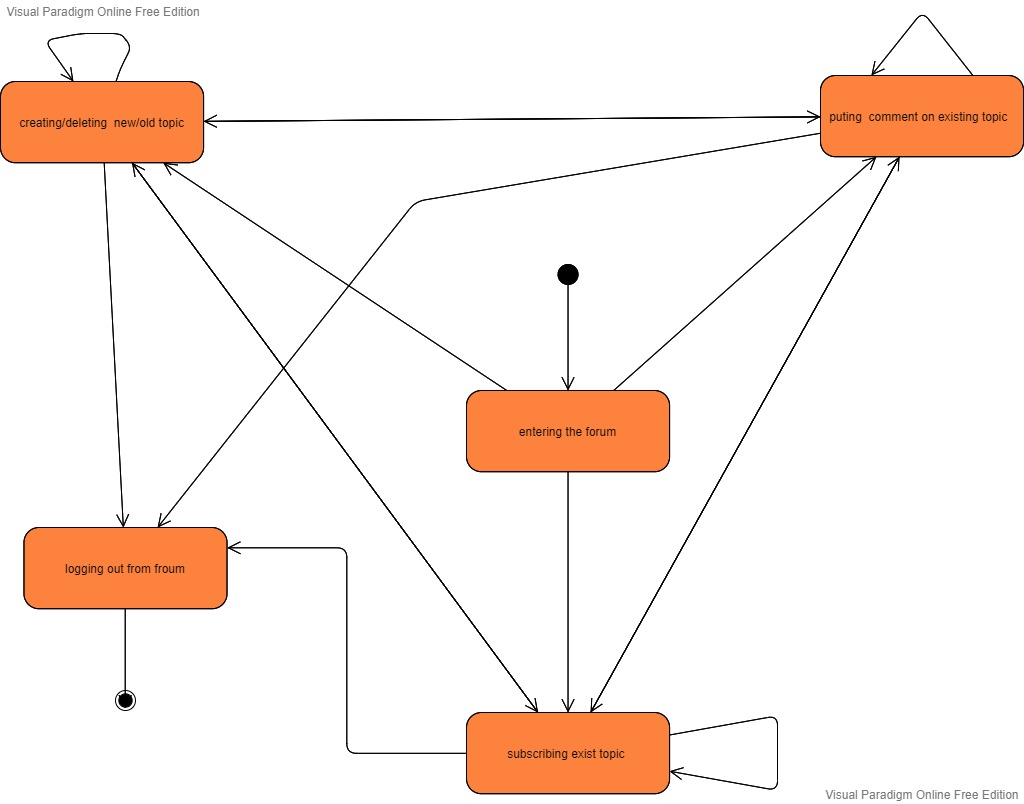
\includegraphics[width=1\textwidth]{figures/SecondStateDiagram.jpg}
\caption{\label{fig:student } State Diagram 2 - communicating in forum with other farmer }
\end{figure}

in the second diagram (figure2), we model how the farmer can communicate with another one,
they can create or delete the  topic, but comment on the topic, and subscribing to existing topics


 \begin{figure}[H]
%\centering
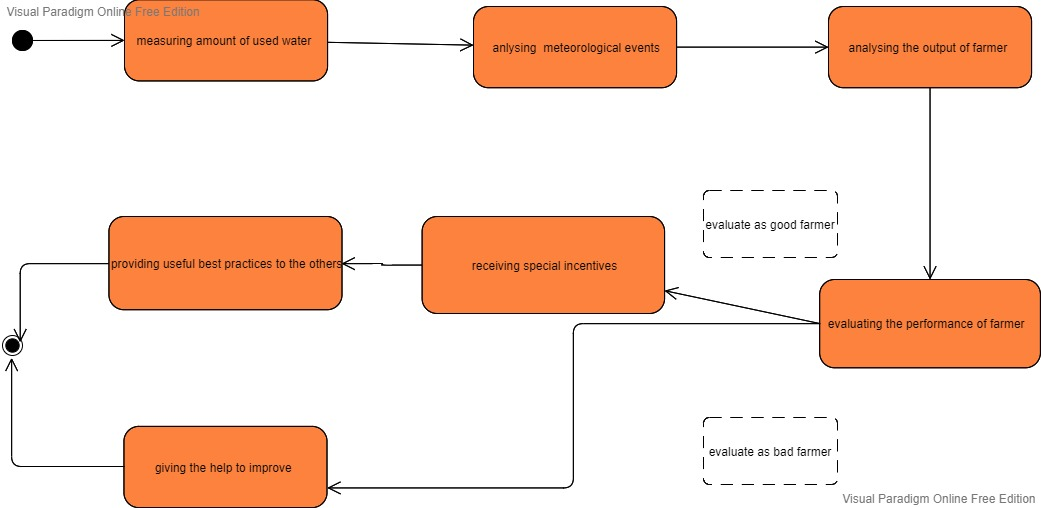
\includegraphics[width=1\textwidth]{figures/thirdStateDiagram.jpg}
\caption{\label{fig:student } State Diagram 3 - evaluate the farmer by policymaker }
\end{figure}
in the third diagram (figure3), we model how the farmers are evaluated by policymakers by using analyzing environmental ones such as meteorological events or used water to identify good farmers to receive incentives or who need to be helped as they are performing particularly badly. 


\pagebreak
\subsection{product function}
Here are described some functions of the software. Be aware that some products functions are described also in other parts of this documents, particularly in the goal parts and in the parts of the functional requirements
 \newline
 \newline
\textbf{give the personalized suggestion}

DREAM, According to collected data such as location, type of production that farmer insert by a farmer in the first step with Weather forecast data collected from
Weather forecast data collected from meteorological stations
by applying the machine learning algorithm, give suggestions to use what crop to plant or specific fertilizers to use.
 \newline
 \newline
\textbf{evaluate the outcome of the agriculturalists}

the service helps policymakers assess the performance of the farmer and determines the best and worst one with collected environmental data, such as the used amount of water measured by irrigation system or humidity of soil obtained from a sensor located in each farmland. Also, consider the type of production and location of land or even what problem the farmer is faced with. The best farmers are encouraged and their opinion is used to improve the performance of others and help those who have not performed well. 
 \newline
 \newline
\textbf{communicate in the forum}

DREAM has a function that lets farmers have communication in the forum and exchange their ideas, comments, problems with other farmers. we should consider that all of these members should be authenticated farmers in our system, consider that farmers can see topics subscribing to them or their own topic and they can put comments on them, also they have the ability to create new topics or delete pre-existed topics which have permissions.






\pagebreak
\subsection{user characteristics}
the actor of the application  are the following :\newline\newline
 1. \textbf{farmer:} who has at least one farmland to produce crop and system help them to improve their capability. a farmer by inserting the type of production, location, Details at work, faced problem has interaction with the system and based on all of this information system besides of environmental factor improve their outcome.\newline
 \newline
 2. \textbf{Policy Maker:}  assess the performance of the farmer and determine the best and worst one with collected environmental data, such as the used amount of water that measure by irrigation system or humidity of soil that obtained from a sensor that located in each farmland  

















\pagebreak

\subsection{Assumption,dependencies and constraints}
\subsubsection{Domain assumption}

\begin{table}[H]
\rowcolors{1}{lightgray}{white}
%\centering
\begin{tabular}{|m{2cm}|l|}
\hline
\normalsize	

D1 & every farmer has at least one land

\\\hline
D2 & every land has sensors to measure the humidity      \\\hline
D3 & the internet connection work properly\\\hline
D4 & farmers insert all of the information about production correctly \\\hline
D5 & farmer insert all of the information correctly \\\hline
D6 & weather forecast ,base on the location is accurate \\\hline
D7 & amount of used water report correctly by irrigation system\\\hline
D8 & police maker asses the former based on true information\\\hline
D9 & just authenticated farmer can send message to forum \\\hline
D10 & amount of reported humidity is correct \\\hline
D11 & farmers insert problems about farm land,production  \\\hline
D12 & in specific location ,there is just one farm land \\\hline
D13 & each user has a smartphone \\\hline
D14 & each smartphone has a GPS sensor integrated  \\\hline 
D15 & GPS is active while app is running \\\hline
D16 & GPS provide the exact location  with an error  of 5 meters at most \\\hline

\hline
\end{tabular}
%\caption{\label{tab:widgets}An example table.}
\end{table}